%% This is based on bare_conf.tex
%% V1.3
%% 2007/01/11
%% by Michael Shell
%% See:
%% http://www.michaelshell.org/
%% for current contact information.
%%
%% This is a skeleton file demonstrating the use of IEEEtran.cls
%% (requires IEEEtran.cls version 1.7 or later) with an IEEE conference paper.
%%
%% Support sites:
%% http://www.michaelshell.org/tex/ieeetran/
%% http://www.ctan.org/tex-archive/macros/latex/contrib/IEEEtran/
%% and
%% http://www.ieee.org/
\documentclass[conference,a4paper]{IEEEtran}

\usepackage{cite}
\usepackage[pdftex]{graphicx}
\usepackage[cmex10]{amsmath}
\usepackage{fixltx2e}
\usepackage{url}

\begin{document}
%
% paper title
% can use linebreaks \\ within to get better formatting as desired
\title{Dynamic Dataflow}

% author names and affiliations
% use a multiple column layout for up to three different
% affiliations
\author{\IEEEauthorblockN{Risto Vuorio}
%\IEEEauthorblockA{Your Association}
}

% make the title area
\maketitle

\begin{abstract}
Dynamic dataflow is a model of computation that is well suited for the
construction of parallel programs. In dynamic dataflow the program logic is
divided into actors that can execute in any order depending only on the data
availability. In most dynamic dataflow implementations the actors are stateless,
which results in a model of computation that resembles functional programming in
many respects.

As the need for high performance parallel computing is growing, dynamic dataflow
based frameworks such as TensorFlow have been introduced to make programming
parallel programs easier. In this paper an introduction to the dynamic dataflow
model of computation is given, the motivation for adoption of the model for
parallel computing is explained and example implementations of the model are
explored.
\end{abstract}

\section{Introduction}
A program following the dataflow model of computation (MoC) consists of a
directed graph with data flowing between the nodes. The data is split into
tokens that are passed between the nodes. The execution of the nodes is
asynchronous. Due to the asynchronous execution the tokens have to be buffered
between the nodes. The dataflow MoC allows for unbounded execution of the model,
which means the dataflow program may execute for a very long time. The
possibility of unbounded execution leads to the problems the different dataflow
MoCs try to solve. A dataflow program capable of unbounded execution 1. may have
unbounded buffer growth 2. if there are cycles, the execution may result in a
deadlock where there are not enough tokens to advance the execution. A good
introduction on the dataflow MoCs is given in \cite{lee2015introduction}.

One popular approach to solving these problems is the synchronous dataflow
(SDF). In SDF the number of tokens produced and consumed by each actor is fixed.
The SDF MoC guarantees bounded buffers and deadlock-free execution but it is
very constrained. For expressing more complicated programs, models with more
design freedom are needed. \cite{lee2015introduction}

There exists a variety of Dataflow MoCs that extend the concept of synchronous
dataflow such as the parameterized and interfaced synchronous dataflow (PiSDF)
\cite{desnos2013pimm}, which extends SDF expressive power by defining parameters
and interfaces. The resulting PiSDF model can be expressed as a SDF. We will not
look at these extensions of SDF but at the more generic Dataflow MoCs
categorized under dynamic dataflow. Dynamic dataflow does not refer to a single
MoC but is rather an umbrella term under which many MoCs fall.

\section{Dynamic Dataflow}
In Dynamic Dataflow (DDF) the number of tokens consumed or produced by an actor
in a single firing is not constrained. An actor can produce and consume
different number of tokens in every firing. This freedom improves the expression
power of the model but makes the analysis more difficult. The difficulty is
underlined by the fact that for the most general class of dataflow models that
bounded buffers and deadlocks are not decidable as proved by Buck
\cite{buck1993scheduling}. It is possible to define dynamic dataflow models that
are decidable by introducing limitations on the types of actors and graph
patterns that can be used in the model \cite{bhattacharyya2013handbook,
gao1992well}. However these limitations are most often traded for the increased
expressive power of the models without such limitations
\cite{bhattacharyya2013handbook}.

Bhattacharyya et al. \cite{bhattacharyya2013handbook} describe many examples of
DDF MoCs. One of these examples is the CAL Actor Language (CAL). CAL is used for
example by the MPEG Reconfigurable Video Coding library. Another example use of
dynamic dataflow is in the TensorFlow (TF) machine learning library by Google
\cite{tensorflow2015-whitepaper}. TF programs are structured as DDF graphs. The
computations in the nodes can be distributed to heterogeneous computing devices
such as CPUs and GPUs. TF provides control flow operators that can be added to
the graph to support conditional execution of parts of the graph and loops.

Dynamic dataflow is a useful model of computation for handling streaming data.
Signal processing applications typically deal with streaming data in the form of
audio, video or other kinds of streams. Streaming data can also be other types
of numeric data, as in the TensorFlow framework, or even textual data as is
often processed in web analytics. The successive and independent dataflow actors
provide logical division of computation for stream processing. The stream
processing context is encountered in the practical use of DDF MoCs
\cite{eker2003cal, tensorflow2015-whitepaper} and in the research where most of
the studies are focused on the performance of either video or audio stream
applications \cite{bhattacharyya2013handbook, roquier2008automatic,
ersfolk2014scheduling}.

Although some of the practical implementations of dynamic dataflow
\cite{tensorflow2015-whitepaper, eker2003cal} allow stateful actors, most of the
dynamic dataflow MoCs presented in \cite{bhattacharyya2013handbook} do not
implement stateful actors to help the analysis of the models. The division of
computation to stateless and independent blocks resembles functional programming
to some extent. This similarity between functional programming and dataflow
models of computation is explored in \cite{reekie1995realtime}.

\subsection{Common Features of DDF Models}
The dynamicity of dynamic dataflow models is introduced through variable number
of input tokens consumed and output tokens produced by the actors
\cite{bhattacharyya2013handbook}. In stateless actors the number of inputs
consumed and outputs produced depends solely on the inputs. The simplest dynamic
actors are the switch and select actors presented in figure \ref{fig:actors1}.
The select actor takes two or more data inputs and a control input. The actor
selects which input to forward to the output port based on the control input. The
switch actor is the counterpart for select, taking only one data input and a
control input. The switch actor outputs its input tokens to the output port
selected with the control input. \cite{lee2015introduction} In the switch and
select actors presented in the figure the number of tokens produced and consumed
on each port is always zero or one but it could be more in some other kind of
actor.

\begin{figure}[!t]
    \centering
        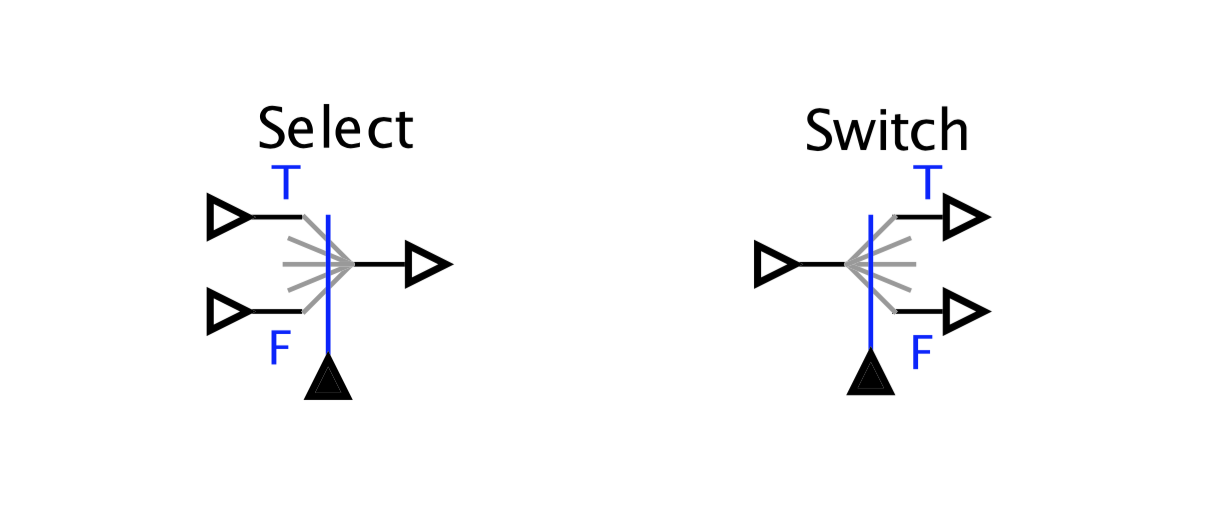
\includegraphics[width=21pc]{ddf_actors.png}
        \caption{Dynamic dataflow switch and select actors. Visualisation from
        \cite{lee2015introduction}}
        \label{fig:actors1}
\end{figure}

From simple conditional actors presented in figure \ref{fig:actors1} dynamic
data paths can be constructed. An example of conditionally executed actors is
presented in figure \ref{fig:conditional}. In the figure actors C and D are
conditionally executed based on the control tokens received from the actor B.
The conditionals provide means for implementing loops and optional data paths in
the dataflow models. These nontrivial extensions improve the expressive power
of the dynamic dataflow models.

\begin{figure}[!t]
    \centering
        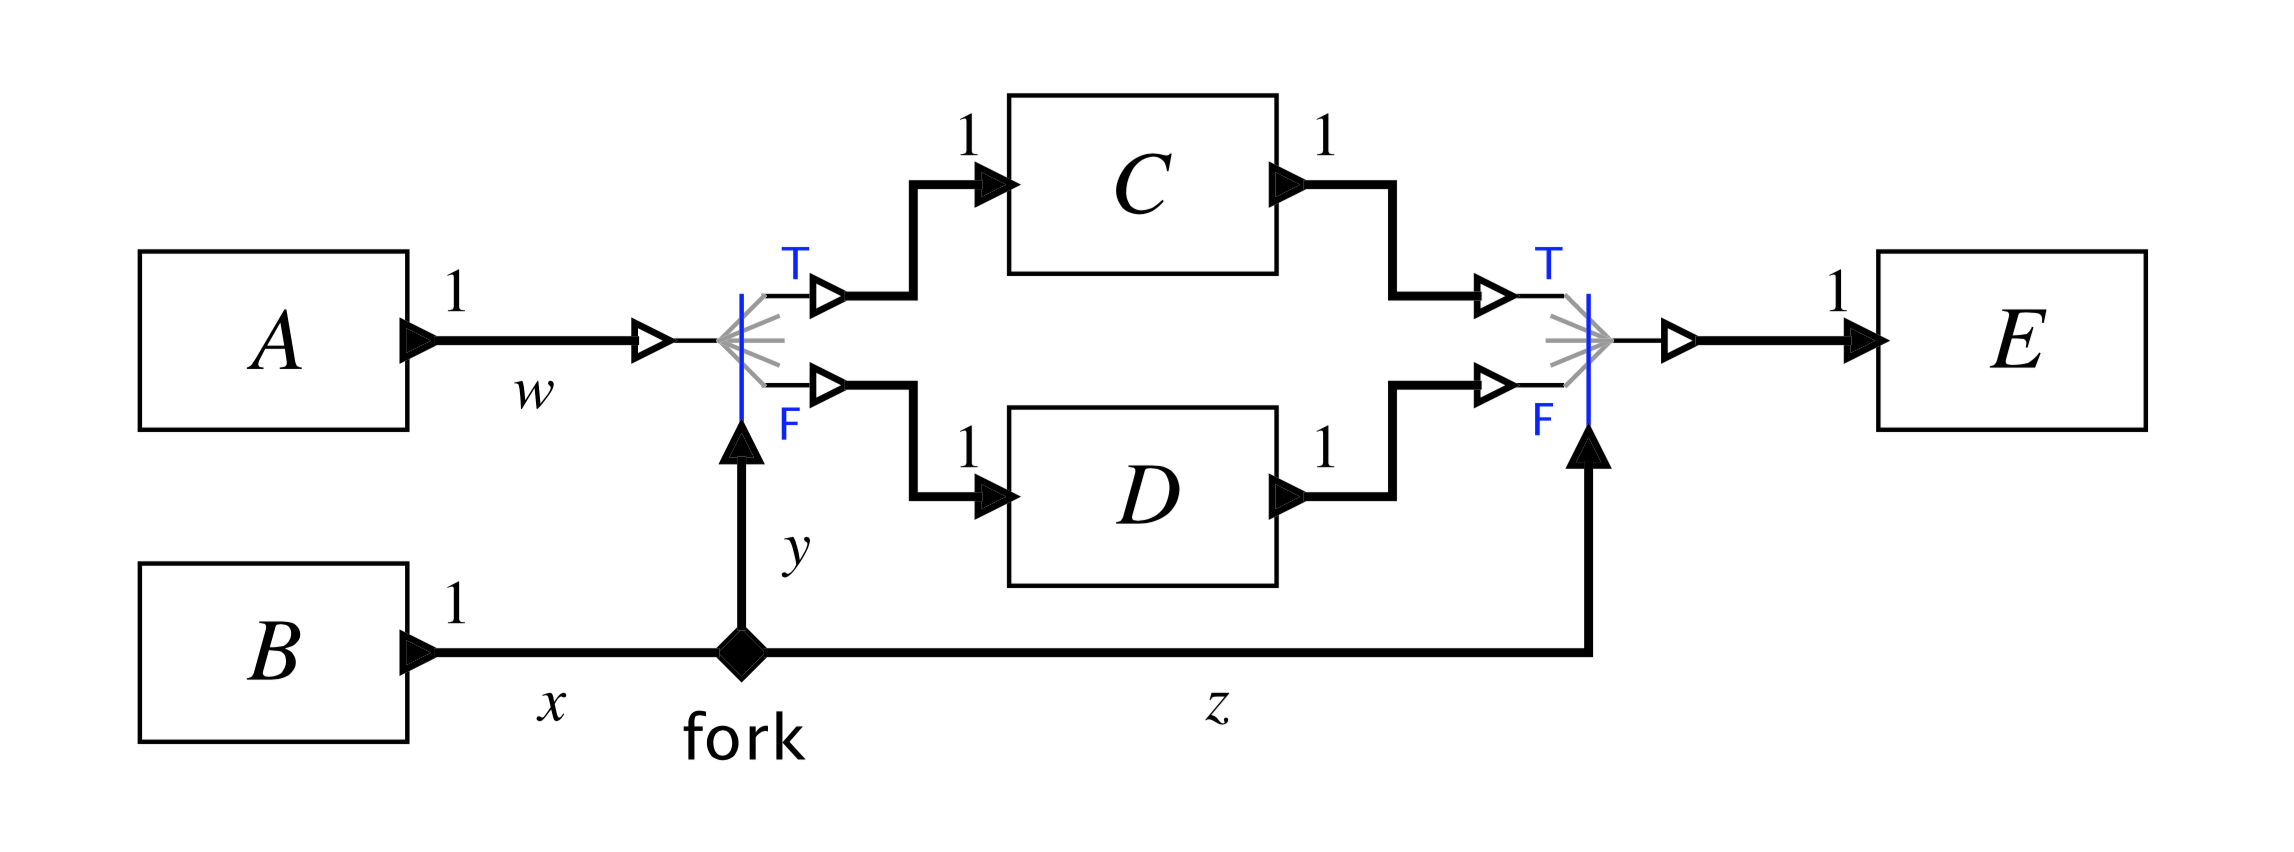
\includegraphics[width=21pc]{ddf_conditional.png}
        \caption{Dynamic dataflow conditional constructed from the switch and
        select actors. Visualisation from \cite{lee2015introduction}}
        \label{fig:conditional}
\end{figure}

\subsection{Scheduling the dynamic dataflow graphs}
As was stated earlier the improved expressive power of the dynamic dataflow
models results in problems with unbounded buffers and the schedulability of the
graphs. Buck \cite{buck1993scheduling} defines scheduling in the context of
dataflow graphs as consisting of three operations. 1. Assigning actors to
processors 2. determining the order of execution of the actors on each processor
3. determining the exact starting time of each actor. The strength of
synchronous dataflow models is that these decisions can be made at compile time.
The dynamic dataflow models need to implement a run time scheduling system.
Especially in signal processing applications the reduced run time overhead and
analysability of compile time scheduling is considered a big advantage.
Therefore there exists dataflow models of computation that combine compile time
and run time scheduling to achieve some of these advantages
\cite{buck1993scheduling, bhattacharyya2013handbook}.

The dynamic scheduling of the dataflow graphs depends on the specific dataflow
model. The basic principle of dynamic scheduling are that actors may execute
after their inputs are available. A naive scheduler could be implemented as a
round-robin that checks the state of each actor in the graph and executes any
actor that has its inputs ready. However this type of scheduler results in
inefficient execution as it does not utilize the structure of the graph to make
scheduling decisions. More sophisticated scheduler implementations are provided
in the different DDF implementations. For example in CAL the graph is first
partitioned in to subgraphs that can be statically scheduled. In some cases
where there are a limited amount of alternative data paths the scheduler may
generate multiple static schedules involving some of the same actors. The
dynamic scheduling decisions are then made between these partitions.
\cite{eker2003cal}

\subsection{Example problems solved using DDF}
The research on dataflow models of computation have been studied extensively for
decades and especially synchronous dataflow has been used in practice as well.
It is no wonder then that the research community has adopted a set of
characteristic examples of the model of computation. The MPEG decoder seems to
be the most commonly studied workload for any new dynamic dataflow model. It is
implemented in CAL \cite{eker2003cal} and SADF \cite{bhattacharyya2013handbook}
to name two examples. MPEG decoder is a well defined but highly complex stream
processing application with practical relevance so it lends itself well to
benchmarking purposes. The MPEG video format achieves compression of the video
data by using motion estimation.

Roughly the video stream is compressed with the following technique. The stream
is encoded into reference frames which represent single frames of the video
stream and predictive-coded frames which represent change from the previous
frames. To decode the stream the difference frames need to be applied on the
reference frames. Dynamicity in the dataflow model of the decoder is introduced
after the input frame is parsed and the type of the frame is determined. The
reference frames and the difference frames are processed differently. Detailed
descriptions of partitioning the MPEG4 decoder into dynamic dataflow graph are
given in \cite{eker2003cal, roquier2008automatic}.

Other example uses of DDF models include encoding and decoding of MP3 audio
format in \cite{bhattacharyya2013handbook} and computing live statistics on
arriving tweets in \cite{murray2013naiad}.

\subsection{TensorFlow}
TensorFlow is a Google framework for machine learning on heterogeneous computing
platforms \cite{tensorflow2015-whitepaper}. The motivation for a variant of
dataflow computing derives from two factors. First the need for efficient means
of construction of parallel programs is only highlighted on heterogeneous
platforms where the computations may take place on different types of
computational units such as CPUs and GPUs and on distributed nodes that are
physically separated.  For practical usability machine learning algorithms need
to be able to handle massive datasets. Many machine learning algorithms break
down into sequential phases of computation that translate into actors naturally.
An simple partial example of a machine learning algorithm represented as a
dataflow graph is presented in figure \ref{fig:simple_tf}.

\begin{figure}[!t]
    \centering
    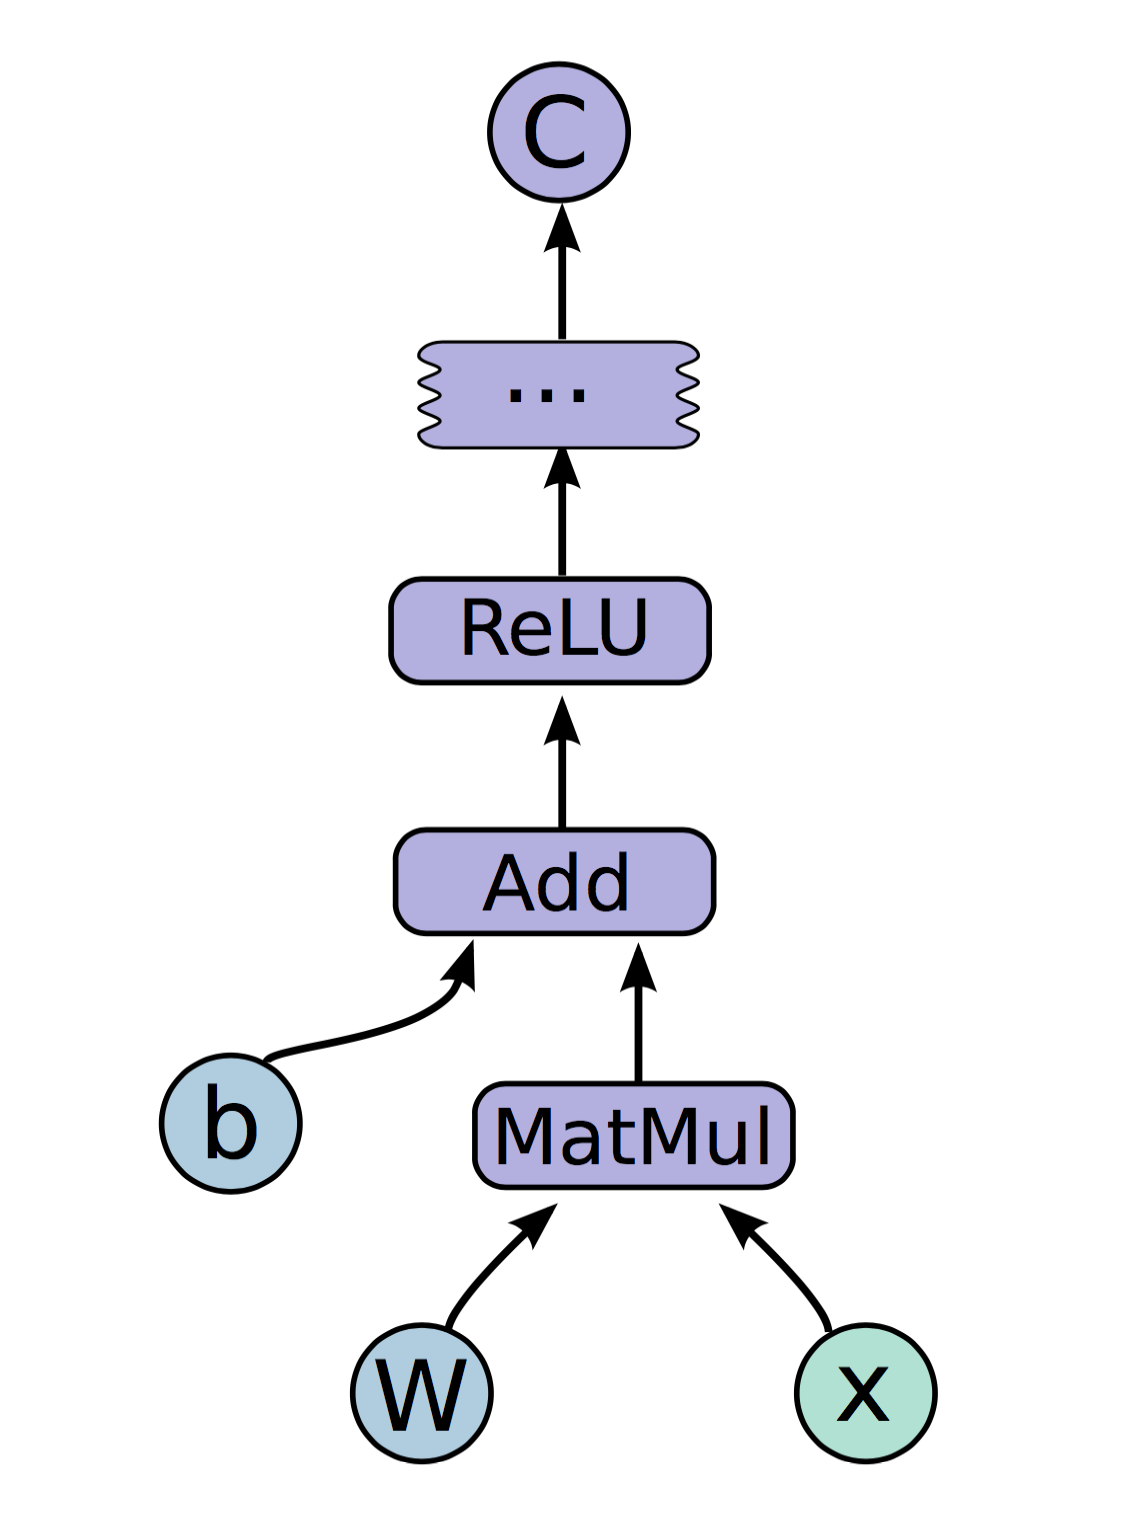
\includegraphics[width=12pc]{tf_simple_neural.png}
        \caption{A partial dataflow graph of a simple neural network. The inputs
        b, W and x are at the bottom of the graph. The rounded rectangles
        represent computation nodes and the output C is at the top. The graph is
        taken from \cite{tensorflow2015-whitepaper}}
        \label{fig:simple_tf}
\end{figure}

The dataflow MoC in TensorFlow is dynamic. Some of the TensorFlow nodes maintain
and update a persistent state. TensorFlow supports loops in the graph, branching
of the graph, conditional execution of nodes and control dependencies. Control
dependencies are edges between the nodes with no data flowing along but they
impose rules on the execution order. If there is a control dependency from node
A to node B, B can not execute before A has completed.
\cite{tensorflow2015-whitepaper}

The TensorFlow runtime schedules the actors on compute devices it has been
configured to use automatically. The open source distribution supports CPUs and
GPUs out-of-the-box. The distributed execution on different host machines is not
currently supported by the open source version. User has additional control of
the asynchronous execution of sub-graphs through the use of queues. The user can
define enqueue and dequeue operations in the graph to utilize queueing features
of the framework. The queues can be used for example for pre-fetching data from
the disk while other part of the graph is using the computational resources.
\cite{tensorflow2015-whitepaper}

\section{Conclusion}
Conclude \\

\bibliographystyle{IEEEtran}
\bibliography{papers}

\end{document}

